% !TEX root=/home/tavant/these/manuscript/src/manuscript.tex

\section{Effect of electron emission}
  \label{sec-see}
  
  In \Cref{sec-canonical}, the walls were not emissive.
  However, the dielectric ceramic used in \ac{HET} can emit electrons \citep{villemant,barral2003a}.
  
  The electron emission model used, introduced in \cref{sec-modelused}, has three parameters $\proba_0, \ek^*, \probamax$, such that the emission probability depends as the kinetic energy of the incident electron $\ek$ as
  \begin{equation} \label{eq-barral_second}
    \proba = \min \lp \proba_0 + (1 -  \proba_0) \frac{\ek}{\ek^*}, \probamax    \rp.
  \end{equation}
  
  The value of parameters are summarized in \cref{tab-tabe_parameters_see}.
  The crossover energy $\ek^*$ is varied from as low as 4~V, corresponding to a very emissive material, to as high as 200~V, a less emissive material.
  
  \begin{table}[hbtp]
  \ra{1.3}
    \centering
    \caption{Parameters of the electron emission probability model}
    \label{tab-tabe_parameters_see}
    \begin{tabular}{@{}ll@{}} \toprule
    Parameter & value  \\ \midrule
    $\proba_0$ & 0.5  \\
    $\probamax$ & 2.9 \\
    $\ek^*$   &  4  -- 200 V\\
    \bottomrule
    \end{tabular}
  \end{table}
  
  \Cref{fig-see_illustration} shows the electron emission probability for $\ek^*=35.04$~V compared to a Maxwellian \ac{EEDF} of temperature of 45~V.
  We can see that the saturation of $\proba$ at $\probamax$ happens only for the very high energy tail.
  
  \begin{figure}[hbtp]
    \centering
    \includegraphics[width=\defaultwidth]{SEE_models}
    \caption{Illustration of the electron emission model of \cref{eq-barral_second} compared to a Maxwellian energy distribution function of temperature of 45~V, with $\ek^*=35.04$~V.}
    \label{fig-see_illustration}
  \end{figure}
  
  In the simulation, we can only measure the average electron emission yield, also named rate, 
  \begin{equation} \label{eq-seeyield}
    \rate = \frac{\Gamma_{\rm emitted}}{\Gamma_{\rm incident}} = \frac{\iiint v_r \proba(\vect{v}) f(\vect{v}) d^3v}{\iiint v_r  f(\vect{v}) d^3v}.
  \end{equation}
  In general, \cref{eq-seeyield} cannot be computed.
  However, if we suppose that the \ac{EEDF} is Maxwellian, \cref{eq-seeyield} can be computed and yields, neglecting the saturation at $\probamax$,
  \begin{equation} \label{eq-seemaxw}
    \ratemaxw(\Te) = \proba_0 + (1 - \proba_0) \frac{2 \Te}{\ek^*}.
  \end{equation}
  \Cref{eq-seemaxw} can be used to estimate the electron emission rate given the mean electron temperature measured in the simulations.
   
  \begin{figure}[hbtp]
    \centering
    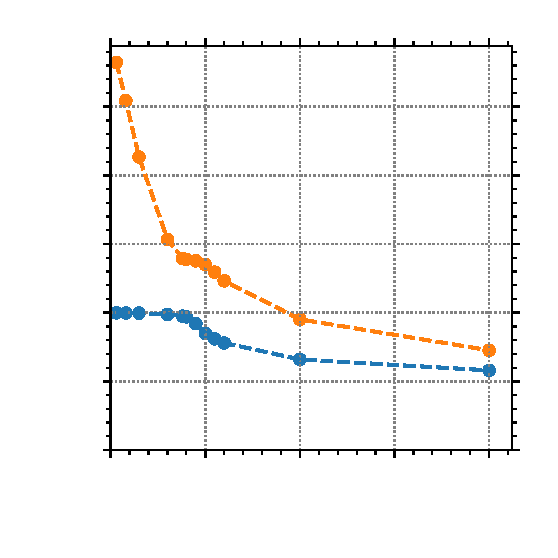
\includegraphics[width=\defaultwidth]{SEE_rates}
    \caption{Values of the electron emission rate $\rate$ (blue) measured in the simulation, and obtained with \cref{eq-seemaxw} using the electron temperature showed in \cref{fig-Tevsproba} }
    \label{fig-seeparamesMaxw}
  \end{figure}
  
  \begin{figure}[hbtp]
    \centering
    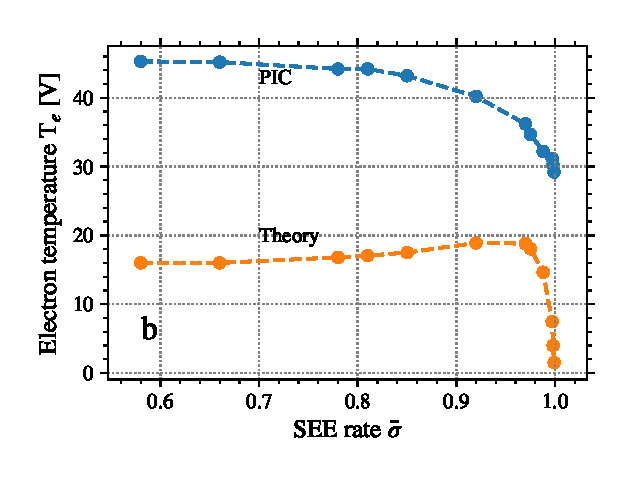
\includegraphics[width=\defaultwidth]{Te_pic_2}
    \caption{Mean electron temperature measured in the \ac{PIC} simulations as a function of the electron emission rate \rate, measured as well in the simulations.  }
    \label{fig-Tevsproba}
  \end{figure}
  
  \Cref{fig-Tevsproba,fig-seeparamesMaxw} show ...
  
  \inlinenote{ Introduce before the "standard" sheath theory with emission }
  
   